\chapter{The Standard Model of Particle Physics}
\label{chap:intro-SM}
%\emph{``I may be bad, but I'm perfectly good at it'' - Rihanna re: the Standard Model (SM), or so I've been told}\\\\

The Standard Model of Particle Physics (SM) is a monumental historical achievement, providing a 
formalism with which one may describe everything from the physics of everyday experience to the 
physics that is studied at very high energies at the Large Hadron Collider (Chapter \ref{chap:experiment}). 
In this chapter, we will provide a brief overview of the pieces that go into the 
construction of such a model. The primary focus of this thesis is searches for pair production of 
Higgs bosons decaying to four $b$-quarks. Consequently, we will pay particular attention to the 
relevant pieces of the Higgs Mechanism, as well as the theory behind searches at a hadronic collider.

\begin{figure}[ht]
  \centering
  \subfloat{
    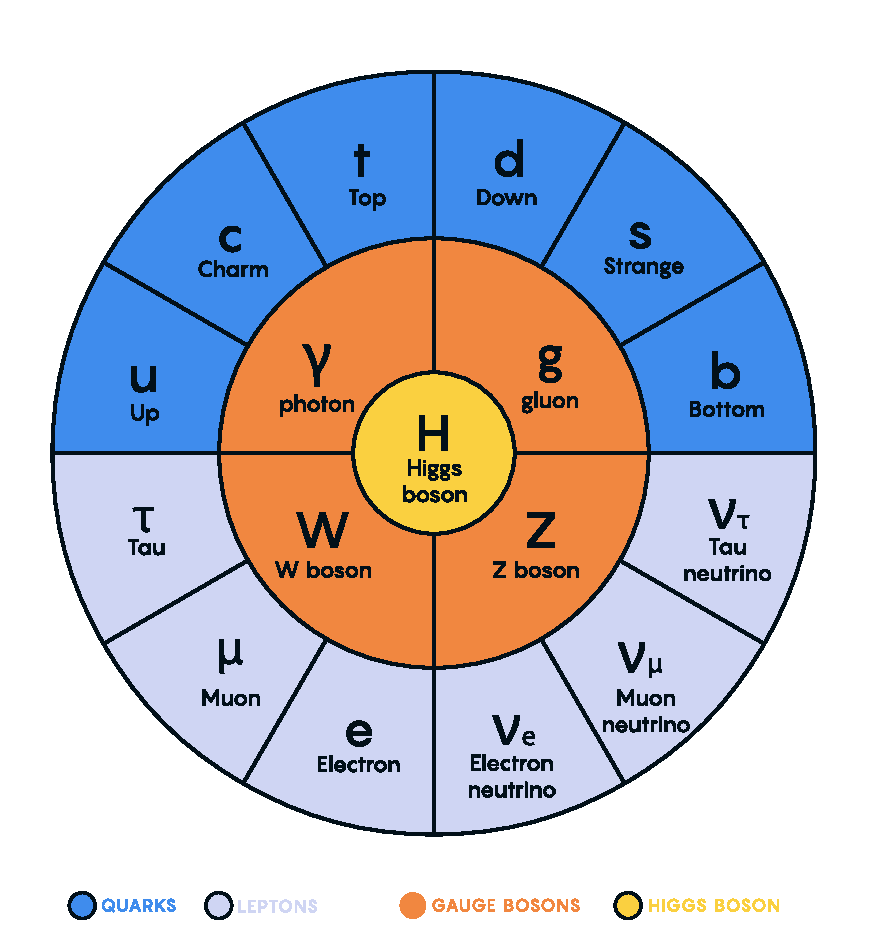
\includegraphics[width=0.8\textwidth]{figures/SM-graphic.pdf}
  }
  \caption{\label{fig:SM-fig} Diagram of the elementary particles described by the Standard Model \cite{SM-figure}.
  }
\end{figure}

\section{Introduction: Particles and Fields}
What is a particle? The Standard Model describes a set of fundamental, point-like, objects shown in Figure \ref{fig:SM-fig}. 
These objects have distinguishing characteristics (e.g., mass and spin). These objects interact in very specific 
ways. The set of objects and their interactions result in a set of observable effects, and these effects are the basis of a field of experimental physics. 

The effects of these objects and their interactions are familiar as fundamental forces: electromagnetism (photons, 
electrons), the strong interaction (quarks, gluons), the weak interaction (neutrinos, $W$ and $Z$ bosons). Gravity is not 
described in this model, as the weakest, with effects most relevant on much larger distance scales than the rest. However, 
the description of these other three is powerful -- verifying and searching for cracks in this description is a large 
effort, and the topic of this thesis.

The formalism for describing these particles and their interactions is that of quantum field theory. Classical field theory is most familiar in the context of, e.g., electromagnetism -- an electric field exists in some region of space, and a charged point-particle experiences a force characterized by the charge of the point-particle and the magnitude of the field at the location of the point-particle in spacetime. The same language translates to quantum field theory. Here, particles are described in terms of quantum fields in some region of spacetime. These fields have associated charges which describe the forces they experience when interacting with other quantum fields. Most familiar is electric charge -- however this applies to e.g., the strong interaction as well, where quantum fields have an associated \emph{color charge} describing behavior under the strong force.

Particles are observed to behave in different ways under different forces. These behaviors respect certain \emph{symmetries}, which are most naturally described in the language of group theory. The respective fields, charges, and 
generators of these symmetry groups are the basic pieces of the SM Lagrangian, which describes the full dynamics of the theory. In the following, we will build up the basic components of this Lagrangian. The treatment presented here 
relies heavily on Jackson's Classical Electrodynamics~\cite{Jackson} for the build-up, and Thomson's Modern Particle 
Physics~\cite{Thomson} for the rest, with reference to Srednicki's Quantum Field Theory~\cite{Srednicki}, and some 
personal biases and interjections.

\FloatBarrier
\section{Quantum Electrodynamics}
Classical electrodynamics is familiar to the general physics audience: electric ($\vec{E}$) and magnetic ($\vec{B}$) 
fields are used to describe behavior of particles with charge $q$ moving with velocity $\vec{v}$, with 
forces described as $\vec{F} =q\vec{E} + q \vec{v} \times \vec{B}$. Hints at some more fundamental properties of
electric and magnetic fields come via a simple thought experiment: in a frame of reference moving along with 
the particle at velocity $\vec{v}$, the particle would appear to be standing still, and therefore have no 
magnetic force exerted. Therefore a \emph{relativistic} formulation of the theory is required. This is most 
easily accomplished with a repackaging: the fundamental objects are no longer classical fields but the electric 
and magnetic \emph{potentials}: $\phi$ and $\vec{A}$ respectively, with
\begin{align}
\vec{E} &= -\grad\phi - \frac{\partial \vec{A}}{\partial t}\\
\vec{B} &= \grad \times \vec{A}
\end{align}

It is then natural to fully repackage into a relativistic \emph{four-vector}: $A^{\mu} = (\phi, \vec{A})$. 
Considering $\partial^{\mu} = (\frac{\partial}{\partial t}, \grad)$, the $x$ components of these above 
two equations become:
\begin{align}
E_{x} &= -\frac{\partial \phi}{\partial x} - \frac{\partial A_{x}}{\partial t} = -( \partial^0 A^1 - \partial^1 A^0)\\
B_{x} &= \frac{\partial A_{z}}{\partial y} - \frac{\partial A_{y}}{\partial z} = -(\partial^2 A^3 - \partial^3 A^2)
\end{align}
where we have used the sign convention $(+, -, -, -)$, such that 
$\partial^{\mu} = (\frac{\partial}{\partial x_0}, -\grad)$.

This is naturally suggestive of a second rank, antisymmetric tensor to describe both the electric and magnetic 
fields (the \emph{field strength tensor}), defined as:
\begin{equation}
F^{\alpha\beta} = \partial^{\alpha}A^{\beta} - \partial^{\beta} A^{\alpha}
\end{equation}

Defining a four-current as $J_{\mu} = (q, \vec{J})$, with $q$ standard electric charge, $\vec{J}$ standard electric 
current, conservation of charge may be expressed via the continuity equation
\begin{equation}
\partial_{\mu}J^\mu = 0
\end{equation}
and all of classical electromagnetism may be packaged into the Lagrangian density:
\begin{equation}
\mathcal{L} = -\frac{1}{4} F_{\mu\nu}F^{\mu\nu} - J^{\mu}A_{\mu}.
\end{equation}

This gets us partway to our goal, but is entirely classical - the description is of classical fields and 
point charges, not of quantum fields and particles. To reframe this, let us go back to the zoomed out view 
of the particles of the Standard Model. Two of the most familiar objects associated with electromagnetism 
are electrons: spin-1/2 particles with charge $e$, mass $m$, and photons: massless spin-1 particles which are
the "pieces" of electromagnetic radiation.

We know that electrons experience electromagnetic interactions with other objects. Given this, and the 
fact that such interactions must be transmitted \emph{somehow} between e.g. two electrons, it seems natural 
that these interactions are facilitated by electromagnetic radiation. More specifically, we may think of 
photons as \emph{mediators} of the electromagnetic force. It follows, then, that a description of 
electromagnetism on the level of particles must involve a description of both the ``source" particles 
(e.g. electrons), the mediators (photons), and their interactions. Further, this description must be 
(1) relativistic and (2) consistent with the classically derived dynamics described above.

The beginnings of a relativistic description of spin-1/2 particles is due to Paul Dirac, with the 
famous Dirac equation:
\begin{equation}
(i\gamma^{\mu}\partial_{\mu} - m)\psi = 0
\end{equation}
where $\partial_{\mu}$ is as defined above, $\psi$ is a Dirac \emph{spinor}, i.e. a four-component 
wavefunction, $m$ is the mass of the particle, and $\gamma^{\mu}$ are the Dirac gamma matrices, 
which define the algebraic structure of the theory. For the following, we also define a conjugate spinor,
\begin{equation}
\bar{\psi} = \psi^{\dagger}\gamma^{0}
\end{equation}
which satisfies the conjgate Dirac equation
\begin{equation}
\bar{\psi}(i\gamma^{\mu}\partial_{\mu} - m) = 0
\end{equation}
where the derivative acts to the left.

The Dirac equation is the dynamical equation for spin-1/2, but we'd like to express these dynamics 
via a Lagrangian density. Further, to have a relativistic description, we'd like to have this be 
density be Lorentz invariant. These constraints lead to a Lagrangian of the form
\begin{equation}
\mathcal{L} = \bar{\psi}(i\gamma^{\mu}\partial_{\mu} - m)\psi 
\end{equation}
where the Euler-Lagrange equation exactly recovers the Dirac equation.


The question now becomes how to marry the two Lagrangian descriptions that we have developed.
Returning for a moment to classical electrodynamics, we know that the Hamiltonian for a charged 
particle in an electromagnetic field is described by 
\begin{equation}
H = \frac{1}{2m}(\vec{p} - q\vec{A})^2 + q\phi.
\end{equation}

Comparing this to the Hamiltonian for a free particle, we see that the modifications required 
are $\vec{p} \rightarrow \vec{p} - q\vec{A}$ and $E\rightarrow E- q\phi$. Using the canonical 
quantization trick of identifying $\vec{p}$ with operator $-i\grad$ and $E$ with operator 
$i\frac{\partial}{\partial t}$, this identification becomes
\begin{equation}
i\partial_{\mu} \rightarrow i\partial_{\mu}-q A_{\mu}
\end{equation}

Allowing for the naive substitution in the Dirac Lagrangian:
\begin{equation}
\mathcal{L} = \bar{\psi}(i\gamma^{\mu}(\partial_{\mu}+iq A_{\mu}) - m)\psi -\frac{1}{4} F_{\mu\nu}F^{\mu\nu}.
\end{equation}
where the source term may be interpreted as coming from the Dirac fields themselves, 
namely, $-q\bar{\psi}\gamma^{\mu}\psi A_{\mu}$.

Setting $q=e$ here (as appropriate for the case of an electron), and defining 
$D_{\mu} \equiv \partial_{\mu} + ieA_{\mu}$, this may then be written in the form
\begin{equation}
\mathcal{L} = \bar{\psi}(i\gamma^{\mu}D_{\mu} - m)\psi -\frac{1}{4} F_{\mu\nu}F^{\mu\nu}.
\end{equation}
which is exactly the quantum electrodynamics Lagrangian.

We have swept a few things under the rug here, however. Recall that the general 
form of a Lagrangian is conventionally $\mathcal{L} = T - V$, where $T$ is the kinetic term, 
and thus ought to contain a derivative with respect to time (c.f. the standard 
$\frac{1}{2}m\frac{\partial x}{\partial t}$ familiar from basic kinematics). More particularly,
given the definition of conjugate momentum as $\partial \mathcal{L}/\partial \dot{q}$ for 
$\mathcal{L}(q, \dot{q}, t)$ and $\dot{q} = \frac{\partial q}{\partial t}$, any field $q$ which 
has no time derivative in the Lagrangian has $0$ conjugate momentum, and thus no dynamics. 

Looking at this final form, there is an easily identifiable kinetic term for the spinor fields (just applying 
the $D_{\mu}$ operator). However trying to identify something similar for the $A$ fields, one 
comes up short -- the antisymmetric nature of $F^{\mu\nu}$ term means that there
is no time derivative applied to $A^0$.

What does this mean? $A^{\mu}$ is a four component object, but it would appear that only three 
of the components have dynamics: we have too many degrees of freedom in the theory. This is the 
principle behind \emph{gauge symmetry} -- an extra constraint on $A^{\mu}$ (a \emph{gauge condition}) 
must be defined such that a unique $A^{\mu}$ defines the theory and satisfies the condition. However, 
we are free to choose this extra condition -- the physics content of the theory should be independent 
of this choice (that is, it should be \emph{gauge invariant}).

To ground this a bit, let us return to basic electric and magnetic fields. These are physical 
quantities that can be measured, and are defined in terms of potentials as 
\begin{align}
\vec{E} &= -\grad\phi - \frac{\partial \vec{A}}{\partial t}\\
\vec{B} &= \grad \times \vec{A}.
\end{align}
It is easy to show, for any scalar function $\lambda$, that $\grad \times \grad\lambda = 0$. This implies 
that the physical $\vec{B}$ field is invariant under the transformation $\vec{A} \rightarrow \vec{A} + \grad\lambda$
for any scalar function $\lambda$.

Under the same transformation of $\vec{A}$, the electric field $\vec{E}$ becomes $-\grad\phi - \frac{\partial \vec{A}}{\partial t} - \frac{\partial \grad\lambda}{\partial t} = -\grad(\phi + \frac{\partial\lambda}{\partial t}) - \frac{\partial\vec{A}}{\partial t}$, such that, for the $\vec{E}$ field to be unchanged, we must additionally apply the transformation 
$\phi \rightarrow \phi - \frac{\partial\lambda}{\partial t}$.

This set of transformations to the potentials that leave the physical degrees of freedom invariant is expressed 
in our four vector notation naturally as
\begin{equation}
A_{\mu} \rightarrow A_{\mu} - \partial_{\mu}\lambda
\end{equation}
where $A_{\mu} = (\phi, -\vec{A})$ with our sign convention. It should be noted that this 
function $\lambda$ is an arbitrary function of \emph{local} spacetime, and thus expresses 
invariance of the physics content under a local transformation.

Let us return to the Lagrangian for QED. In particular, focusing on the free Dirac piece
\begin{equation}
\mathcal{L} = \bar{\psi}(i\gamma^{\mu}\partial_{\mu} - m)\psi 
\end{equation}
we note that if we apply a local transformation of the form $\psi\rightarrow e^{iq\lambda(x)}\psi$
(and correspondingly $\bar{\psi}\rightarrow \bar{\psi}e^{-iq\lambda(x)}$, by definition), the Lagrangian 
becomes
\begin{equation}
\bar{\psi}e^{-iq\lambda(x)}(i\gamma^{\mu}\partial_{\mu} - m)e^{iq\lambda(x)}\psi = 
\bar{\psi}e^{-iq\lambda(x)}(i\gamma^{\mu}\partial_{\mu})e^{iq\lambda(x)}\psi - m\bar{\psi}\psi.
\end{equation}
As $\partial_{\mu} (e^{iq\lambda(x)}\psi) = iqe^{iq\lambda(x)}(\partial_{\mu}\lambda(x))\psi + e^{iq\lambda(x)}\partial_{\mu}\psi$, this becomes
\begin{equation}
\bar{\psi}(i\gamma^{\mu}(\partial_{\mu}+iq\partial_{\mu}\lambda(x)) - m)\psi.
\end{equation}
Thus, the free Dirac Lagrangian on its own is not invariant under this transformation. We may note, however,
that on interaction with an electromagntic field, as described above, this transformed Lagrangian
may be packaged as:
\begin{equation}
\bar{\psi}(i\gamma^{\mu}(\partial_{\mu}+ iq\partial_{\mu}\lambda(x)+iq A_{\mu}) - m)\psi =
\bar{\psi}(i\gamma^{\mu}(\partial_{\mu}+ iq(A_{\mu}+\partial_{\mu}\lambda(x)) - m)\psi.
\end{equation}
since by the arguments above, the physics content of the Lagrangian is invariant under the transformation 
$A_{\mu} \rightarrow A_{\mu} - \partial_{\mu}\lambda$,  we may directly make this transformation, and remove 
this extra $\partial_{\mu}\lambda(x)$ term. It is straightforward to verify that the $\frac{1}{4} F_{\mu\nu}F^{\mu\nu}$
term is invariant under this same transformation of $A_{\mu}$, so we may say that the QED Lagrangian is 
invariant under local transformations of the form $\psi\rightarrow e^{iq\lambda(x)}\psi$.

These arguments illuminate some important concepts which will serve us well going forward. First, while we have 
remained grounded in the ``familiar'' physics of electromagnetism for the above, arguments of the ``top down''
variety would lead us to the exact same conclusions. That is, suppose we wanted to construct a theory of 
spin-1/2 particles that was invariant under local transformations of the form $\psi\rightarrow e^{iq\lambda(x)}\psi$. 
More broadly, we could say that we desire this theory to be invariant under local $U(1)$ transformations, where 
$U(1)$ is exactly this group, under multiplication, of complex numbers with absolute value 1. By very similar 
arguments as above, we would see that, to achieve invariance, this theory would necessitate an additional degree 
of freedom, $A_{\mu}$, with the exact properties that are familiar to us from electrodynamics. These arguments 
based on symmetries are extremely powerful in building theories with a less familiar grounding, as we will 
see in the following.

Second, we defined this quantity $D_{\mu} \equiv \partial_{\mu} + ieA_{\mu}$ above, seemingly as a matter 
of notational convenience. However, from the latter set of arguments, such a packaging takes on a new power: 
by explicitly including this gauge field $A_{\mu}$ which transforms in such a way as to keep invariance 
under a given transformation, the invariance is immediately more manifest. That is, to pose the $U(1)$ 
invariance in a more zoomed out way, under the transformation $\psi\rightarrow e^{iq\lambda(x)}\psi$,
while
\begin{equation}
\bar{\psi}\partial_{\mu}\psi \rightarrow \bar{\psi}(\partial_{\mu}+iq\partial_{\mu}\lambda(x))\psi
\end{equation}
with the extra term that gets canceled out by the gauge transformation of $A_{\mu}$,
\begin{equation}
\bar{\psi}D_{\mu}\psi \rightarrow \bar{\psi}D_{\mu}\psi
\end{equation}
where this transformation is already folded in. This repackaging, called a \emph{gauge covariant derivative} 
is much more immediately expressive of the symmetries of the theory.

Finally, to emphasize how fundamental these gauge symmetries are to the corresponding theory, let us examine
the additional term needed for $U(1)$ invariance, $q\bar{\psi}\gamma^{\mu}A_{\mu}\psi$. While a first principles
examination of Feynman rules is beyond the scope of this thesis, it is powerful to note that this is expressive 
of a QED vertex: the $U(1)$ invariance of the theory and the interaction between photons and electrons are 
inextricably tied together.

\section{An Aside on Group Theory}
Quantum electrodynamics is very familiar and well covered, and provides (both historically and in this thesis) 
a nice bridge between ``standard'' physics and the language of symmetries and quantum field theory. However, now 
that we are acquainted with the language, we may set up to dive a bit deeper. To begin, let us look again at the $U(1)$ 
group that is so fundamental to QED. We have expressed this via a set of transformations on our Dirac spinor objects, 
$\psi$, of the form $e^{iq\lambda(x)}$. Note that such transformations, though they are local (i.e. a function of 
spacetime) are purely \emph{phase} transformations. Relatedly, $U(1)$ is an Abelian group, meaning that 
group elements commute.

To set up language to generalize beyond $U(1)$, note that we may equivalently write $U(1)$ elements as
$e^{ig\vec{\alpha}(x)\cdot \vec{T}}$, $\vec{\alpha}(x)$ and $\vec{T}$ and are vectors in the space of 
\emph{generators} of the group, with each $\alpha^{a}(x)$ an associated scalar function to generator $t^{a}$, 
and $g$ is some scalar strength parameter. Of course this is a bit silly for $U(1)$, which has a single generator, 
and thus reduces to the transformation we discussed above. However, this becomes much more useful for groups of higher 
degree, with more generators and degrees of freedom.

To discuss these groups in a bit more detail, note that $U(n)$ is the unitary group of 
degree $n$, and corresponds to the group of $n \times n$ unitary matrices (that is, $U^{\dagger}U = UU^{\dagger} = 1$).
Given that group elements are $n\times n$, this means that there are $n^2$ degrees of freedom:
$n^2$ generators are needed to characterize the group.

For $U(1)$, this is all consistent with what we have said above -- the group of $1 \times 1$ unitary matrices 
have a single generator, and the phases we identify above clearly satisfy unitarity. Note that these degrees 
of freedom for the gauge group also characterize the number of gauge bosons we need to satisfy the local symmetry: 
for $U(1)$, we need one gauge boson, the photon.

Of relevance for the Standard Model are also the special unitary groups $SU(n)$. These are defined similarly 
to the unitary groups, with the additional requirement that group elements have determinant $1$. This extra 
constraint removes $1$ degree of freedom: groups are characterized by $n^2-1$ generators.

In particular, we will examine the groups $SU(2)$ in the context of the weak interaction, with an associated
$2^2-1=3$ gauge bosons (cf. the $W^{\pm}$ and $Z$ bosons), and $SU(3)$, with an associated $3^2-1 = 8$ gauge bosons 
(cf. gluons of different flavors). Note that these groups are non-Abelian ($2\times 2$ or $3\times 3$ matrices do not, 
in general, commute), leading to a variety of complications. However, both of these theories feature interactions with 
spin-1/2 particles, with transformations of a very similar form: $\psi \rightarrow e^{ig\vec{\alpha}(x)\cdot \vec{T}}\psi$, 
and the general framing of the arguments for QED will serve us well in the following.


\section{Quantum Chromodynamics}
In some sense, the simplest extension the development of QED is quantum chromodynamics (QCD). QCD is a 
theory in which, once the basic dynamics are framed (a non-trivial task!) the group structure becomes 
apparent. The quark model, developed by Murray Gell-Mann~\cite{Gell-Mann} and George Zweig~\cite{Zweig}, provided the 
fundamental particles involved in the theory, and had great success in explaining the expanding zoo 
of experimentally observed hadronic states.

Some puzzles were still apparent -- the $\Delta^{++}$ baryon, e.g., is composed of three up quarks, 
$u$, with aligned spins. As quarks are fermions, such a state should not be allowed by the Pauli exclusion 
principle. The existence of such a state in nature implies the existence of another quantum number, and 
a triplet of values, called \emph{color charge} was proposed by Oscar Greenberg~\cite{Greenberg}. With these
pieces in place, the structure becomes more apparent, as elucidated by Han and Nambu~\cite{Han-Nambu}.

Let us reason our way to the symmetries using color charge. Experimentally, we know that there is this triplet
of color charge values $r, g, b$ (the ``plus'' values, cf. electric charge) and correspondingly anti-color charge
$\bar{r}, \bar{g}, \bar{b}$ (the ``minus'' values). Supposing that the force behind QCD (the \emph{strong force}) is, 
similar to QED, interactions between fermions mediated by gauge bosons (quarks and gluons respectively), we can 
start to line up the pieces.

What color charge does a gluon have? Similarly to electric charge, we may associate particles
with color charge, anti-particles with anti-color charge. Notably, free particles observed experimentally are 
colorless (have no color charge). Thus, in order for charge to be conserved throughout such 
processes, this already implies that there are charged gluons. Further, examining color flow diagrams 
such as \todo{insert}, it is apparent first that a gluon has not one but two associated color charges
and second that these two must be one color charge and one anti-color charge.

Counting up the available types of gluons, then, we come up with nine. Six of mixed color type: 
$r\bar{b}, r\bar{g}, b\bar{r}, b\bar{g}, g\bar{b}$, and $g\bar{r}$, and three of same color type:
$r\bar{r}$, $g\bar{g}$, and $b\bar{b}$. In practice, however, these latter three are a bit redundant:
all express a colorless gluon, which, if we could observe this as a free particle, would be indistinguishable
from each other. The \emph{color singlet} state is then a mix of these, $\frac{1}{\sqrt{3}}(r\bar{r}+g\bar{g}+b\bar{b})$,
leaving two unclaimed degrees of freedom, which may be satisfied by the linearly independent combinations
$\frac{1}{\sqrt{2}}(r\bar{r}-g\bar{g})$ and $\frac{1}{\sqrt{6}}(r\bar{r}+g\bar{g}-2b\bar{b})$.

We thus have an octet of color states plus a colorless singlet state. If this colorless singlet state 
existed, however, we would be able to observe it, not only via interactions with quarks, but as a free
particle. Since do not observe this in nature, this restricts us to $8$ gluons. The simplest group with 
a corresponding 8 generators is $SU(3)$. Under the assumption that $SU(3)$ is the local gauge symmetry
of the strong interaction, we may proceed in a similar way as we did for QED. The gauge transformation is 
$\psi \rightarrow e^{ig_{S}\vec{\alpha}(x)\cdot \vec{T}}\psi$, where $\vec{T}$ is an eight component vector
of the generators of $SU(3)$, often expressed via the Gell-Mann matrices, $\lambda^{a}$, as $t^{a} = \frac{1}{2}\lambda^{a}$,
and the spinor $\psi$ represents the fields corresponding to quarks.

This $SU(3)$ symmetry exactly expresses the color structure elucidated above -- the Gell-Mann matrices are an 
equivalent presentation of the color combinations described above. Proceeding by analogy to QED, gauge invariance 
is achieved by introducing eight new degrees of freedom, $G_{\mu}^{a}$, which are the gauge fields corresponding to 
the gluons, with the gauge covariant derivative then analogously taking the form 
$D_{\mu} \equiv \partial_{\mu} + ig_{S}G_{\mu}^{a}t^{a}$.

Recall from the QED derivation that the field strength tensor, $F^{\mu\nu}$ is a rank two antisymmetric
tensor which is manifestly gauge invariant and which describes the physical dynamics of the $A_{\mu}$ field.
We would like to analogously define a term for the gluon fields. Repackaging this QED tensor, it is apparent that
\begin{align}
[D_{\mu}, D_{\nu}] &= D_{\mu}D_{\nu} - D_{\nu}D_{\mu}\\
&= (\partial_{\mu} + iqA_{\mu})(\partial_{\nu} + iqA_{\nu}) - (\partial_{\nu} + iqA_{\nu})(\partial_{\mu} + iqA_{\mu})\\
&= \partial_{\mu}\partial_{\nu}+iq\partial_{\mu}A_{\nu} + iqA_{\mu}\partial_{\mu} + (iq)^2A_{\mu}A_{\nu} -
(\partial_{\nu}\partial_{\mu}+iq\partial_{\nu}A_{\mu} + iqA_{\nu}\partial_{\nu} + (iq)^2A_{\nu}A_{\mu})\\
&=iq(\partial_{\mu}A_{\nu}-\partial_{\nu}A_{\mu}) + (iq)^2(A_{\mu}A_{\nu}-A_{\nu}A_{\mu})\\
&=iq(\partial_{\mu}A_{\nu}-\partial_{\nu}A_{\mu})+(iq)^2[A_{\mu}, A_{\nu}].
\end{align}

We proceed through this derivation to highlight that, in the specific case of QED, with its Abelian $U(1)$ gauge
symmetry, the field commutator vanishes, leaving exactly the definition of $F_{\mu\nu}$ as described above, i.e.,
\begin{equation}
F_{\mu\nu} = \frac{1}{iq}[D_{\mu}, D_{\nu}].
\end{equation}

We may proceed to define an analagous field strength term for $G_{\mu}^{a}$ in a similar way:
\begin{equation}
G_{\mu\nu} = \frac{1}{ig_{S}}[D_{\mu}, D_{\nu}]
\end{equation}
This has an extremely nice correspondence, but is complicated by the non-Abelian nature of $SU(3)$, with
\begin{equation}
G_{\mu\nu} = \partial_{\mu}(G_{\nu}^{a}t^{a}) - \partial_{\nu}(G_{\mu}^{a}t^{a}) + ig_{s}[G_{\mu}^{a}t^{a}, G_{\nu}^{a}t^{a}].
\end{equation}
in which the field commutator term is non-zero. In particular (since each term is summing over $a$, so we may relabel) as
\begin{equation} 
[G_{\mu}^{a}t^{a}, G_{\nu}^{b}t^{b}] = [t^{a}, t^{b}]G_{\mu}^{a}G_{\nu}^{b}
\end{equation}
and as $[t^{a}, t^{b}] = if^{abc}t^c$ for the Gell-Mann matrices, where $f^{abc}$ are the structure
constants of $SU(3)$, we have
\begin{align}
G_{\mu\nu} &= \partial_{\mu}(G_{\nu}^{a}t^{a}) - \partial_{\nu}(G_{\mu}^{a}t^{a}) -g_{s}f^{abc}t^cG_{\mu}^{a}G_{\nu}^{b}\\
&=t^{a}(\partial_{\mu}G_{\nu}^{a}-\partial_{\nu}G_{\mu}^{a}-f^{bca}G_{\mu}^{b}G_{\nu}^{c})\\
&=t^{a}G_{\mu\nu}^a
\end{align}
for $G_{\mu\nu}^a = \partial_{\mu}G_{\nu}^{a}-\partial_{\nu}G_{\mu}^{a}-f^{abc}G_{\mu}^{b}G_{\nu}^{c}$.

This gives the component of the field strength corresponding to a particular gauge field $a$, where 
the first two terms have the familiar form of the QED field strength, while the last term is new, and 
explicitly related to the group structure via the $f^{abc}$ constants. In terms of the physics content of the 
theory, this latter term gives rise to a gluon \emph{self-interaction}, a distinguishing feature of QCD.

Similarly as in QED, a Lorentz invariant combination of field strength tensors may be made as $G_{\mu\nu}G^{\mu\nu}$.
However, this is not manifestly gauge invariant. Under a gauge transformation $U$, the covariant derivative 
behaves as $D^{\mu}\rightarrow UD^{\mu}U^{-1}$, corresponding to $G^{\mu\nu}\rightarrow UG^{\mu\nu}U^{-1}$.
The cyclic property of the trace thus ensures the gauge invariance of $\tr(G_{\mu\nu}G^{\mu\nu})$, which we 
will write as $G_{\mu\nu}^a G^{\mu\nu}_a$ with the implied sum over generators $a$.

Packaging up the theory, it is tempting to copy the form of the QED Lagrangian,
with the identifications we have made above:
\begin{equation}
\mathcal{L} = \bar{\psi}(i\gamma^{\mu}D_{\mu} - m)\psi -\frac{1}{4} G_{\mu\nu}^{a}G^{\mu\nu}_{a}.
\end{equation}
However this is not quite correct due to the $SU(3)$ nature of the theory. In terms of the physics,
the Dirac fields $\psi$ have associated color charge, which must interact appropriately with the 
$G_{\mu}$ fields. Mathematically, the generators $t^{a}$ are $3\times 3$ matrices, while the $\psi$ are
four component spinors. Adding a color index to the Dirac fields, i.e., $\psi_{i}$ where $i$ runs over 
the three color charges, and similarly indexing the generators $t_{ij}^{a}$, we may then express the 
$SU(3)$ gauge covariant derivative component-wise as 
\begin{equation}
(D_{\mu})_{ij} = \partial_{\mu}\delta_{ij} + ig_{S}G_{\mu}^{a}t^{a}_{ij}
\end{equation}
where $\delta_{ij}$ is the Kronecker delta, as $\partial_{\mu}$ does not participate in the $SU(3)$
structure.

The Lagrangian then becomes
\begin{equation}
\mathcal{L} = \bar{\psi}_{i}(i(\gamma^{\mu}D_{\mu})_{ij} - m\delta_{ij})\psi_{j} -\frac{1}{4} G_{\mu\nu}^{a}G^{\mu\nu}_{a}.
\end{equation}

and we have constructed QCD.


\section{The Weak Interaction}
One of the first theories of the weak interaction was from Enrico Fermi~\cite{Fermi}, in an effort to 
explain beta decay, a process in which an electron or positron is emitted from an atomic nucleus, resulting 
in the conversion of a neutron to a proton or proton to a neutron respectively. Fermi's hypothesis was 
of a direct interaction between four fermions. However, in the advent of QED, it is natural to wonder if 
a theory of based on mediator particles and gauge symmetries applies to the weak force as well. The modern formulation 
of such a theory is due to Sheldon Glashow, Steven Weinberg, and Abdus Salam ~\cite{Glashow}, and is what we will 
describe in the following.

Considering emission of an electron, Fermi's theory involves an initial state neutron that transitions 
to a proton with the emission of an electron and a neutrino. This transition gives a hint that something 
slightly more complicated is happening than in QED: there is an apparent mixing between particle types. 

Now, with the assumption there are mediators for such an interaction, we further know from beta decay and 
charge conservation that there must be at least two such degrees of freedom: e.g. one that decays to an electron 
and neutrino ($W^{-}$) and one that decays to a positron and neutrino ($W^{+}$). From consideration of the process 
$e^{+}e^{-}\rightarrow W^{+}W^{-}$, it turns out that with just these two degrees of freedom, the cross section for this process increases without limit as a function of center-of-mass energy, ultimately violating unitarity (more $W^{+}W^{-}$ 
pairs come out than $e^{+}e^{-}$ pairs go in). This is resolved with a third, neutral degree of freedom, the $Z$
boson, whose contribution interferes negatively, regulating this process.

This leads to three degrees of freedom for the gauge symmetry of the weak interactions, so we thus need a theory 
which is locally invariant under transformations of a group with three generators. The simplest such choice is $SU(2)$. 
We may follow a very similar prescription as for QED and QCD: $SU(2)$ has three generators, which implies the existence of 
three gauge bosons, call them $W_{\mu}^k$.  The gauge transformation may be expressed as $\psi \rightarrow e^{ig_{W}\vec{\alpha}(x)\cdot \vec{T}}\psi$, where in this case the generators are for $SU(2)$, which may be written in terms of the familiar
Pauli matrices: $\vec{T} = \frac{1}{2}\vec{\sigma}$. The structure constants for $SU(2)$ are the antisymmetric Levi-Civita 
tensor, so the corresponding gauge covariant derivative is
$D_{\mu} \equiv \partial_{\mu} + ig_{W}W_{\mu}^{k}t^{k}$, and the field strength tensor is 
$W_{\mu\nu}^{k} = \partial_{\mu}W_{\nu}^{k}-\partial_{\nu}W_{\mu}^{k}-\epsilon^{ijk}W_{\mu}^{k}W_{\nu}^{k}$.

The corresponding Lagrangian would thus be
\begin{equation}
\mathcal{L} = \bar{\psi}_{i}(i(\gamma^{\mu}D_{\mu})_{ij} - m\delta_{ij})\psi_{j} -\frac{1}{4} W_{\mu\nu}^{k}W^{\mu\nu}_{k}
\end{equation}
where indices $i$ and $j$ run over $SU(2)$ charges.

On considering some of the details, the universe unfortunately turns out to be a bit more complicated. However, this still
provides a useful starting place for elucidating the theory of weak interactions. First off, let us consider the 
particle content, namely, what do the Dirac fields correspond to? This is still a theory of fermionic interactions
with gauge bosons. However, we might notice that the fermion content of this theory is both a) broader than QCD, 
as we know experimentally (cf. beta decay) that both quarks and leptons (e.g. electrons) participate in the 
weak interaction and b) this fermion content seemingly has a large overlap with QED. In terms of the gauge bosons, 
we know that at both $W^{+}$ and $W^{-}$ are electrically charged -- this means that we expect some interaction of 
the weak theory with electromagnetism. 

However, before diving deeper into this apparent connection between the weak interaction and QED, let us focus on the
gauge symmetry. In QCD, the $SU(3)$ content of the theory is expressed via a contraction of color indices -- the theory 
allows for transitions between quarks of one color and quarks of another. Thinking similarly in terms of $SU(2)$ transitions,
the beta decay example is already fruitful -- there is a transition between an electron and its corresponding neutrino, 
as well as between two types of quark. In particular, for the case of neutron (with quark content $udd$) and proton 
(with quark content $udu$), the weak interaction provides for a transtion from down to up quark.

Such $SU(2)$ dynamics are described via a quantity called \emph{weak isospin}, denoted $I_{W}$ with third component 
$I_{W}^{(3)}$, and can be thought of in a very similar way as color charge in QCD (i.e. as the charge corresponding to the 
weak interaction). Since $SU(2)$ is $2 \times 2$, there are two such charge states for the fermions, denoted as 
$I_{W}^{(3)}=\pm \frac{1}{2}$. This means that the bosons must have $I_{W} = 1$ such that, by sign convention corresponding 
to electric charge, the $W^{+}$ boson has $I_{W}^{(3)}=+1$, the $Z$ boson has $I_{W}^{(3)}=0$, and the $W^{-}$ boson has
$I_{W}^{(3)}=-1$.

From conservation of electric charge, this means that transitions involving a $W^{\pm}$ are between particles that differ by
$\pm 1$ in both weak isospin $I_{W}^{(3)}$ and electric charge. We may thus line up all such doublets as: 
\begin{equation}
\begin{pmatrix}\nu_{e} \\ e^{-}\end{pmatrix}, \begin{pmatrix}\nu_{\mu} \\ \mu^{-}\end{pmatrix}, 
\begin{pmatrix}\nu_{\tau} \\ \tau^{-}\end{pmatrix}, \begin{pmatrix}u \\ d'\end{pmatrix}, 
\begin{pmatrix}c \\ s'\end{pmatrix}, \begin{pmatrix}t \\ b'\end{pmatrix}
\end{equation}
with the top corresponding to the lower weak isospin and electric charge particles, and the lower quark entries 
($d'$, etc) corresponding to the weak quark eigenstates (which are related to the mass eigenstates by the CKM 
matrix \todo{more detail}). Similar doublets may be constructed for the corresponding anti-particles.

The fundamental structuring of these transitions around both electric and weak charge is again indicative of a natural 
connection. However, nature is again a bit more complicated than we have described. This is because the weak interaction
is a \emph{chiral} theory. For massless particles, chirality is the same as the perhaps more intuitive \emph{helicity}. 
This describes the relationship between a particle's spin and momentum: if the spin vector points in the same 
direction as the momentum vector, helicity is positive (the particle is ``right-handed''), and if the two point 
in opposite directions, the helicity is negative (the particle is ``left-handed''). More concretely:
\begin{equation}
H = \frac{\vec{s}\cdot\vec{p}}{|\vec{s}\cdot \vec{p}|}.
\end{equation}

For massive particles, this generalizes a bit -- in the language of Dirac fermions that we have developed, 
we define projection operators
\begin{equation}
P_{R} = \frac{1}{2}(1+\gamma^{5}) \hspace{0.2in}\text{and}\hspace{0.2in}P_{L} = \frac{1}{2}(1-\gamma^{5}) 
\end{equation}
for right and left-handed chiralities respectively -- acting on a Dirac field with such operators 
projects the field onto the corresponding chiral state.

Experimentally, this pops up via parity violation and the famous $V - A$ theory. 
For the scope of this thesis, it is sufficient to say that the weak interaction is only observed to take
place for left-handed particles (and correspondingly, right-handed anti-particles). We therefore modify the 
theory stated above by projecting all fermions participating in the weak interaction onto respective chiral
states -- in particular, the $SU(2)$ gauge symmetry only acts on left-handed particles and right-handed anti-particles.
We therefore modify the theory appropriately, denoting the chiral projected gauge symmetry as $SU(2)_{L}$, 
and similarly for the Dirac fields. In particular, the weak isospin doublets listed above must now be 
left-handed:
\begin{equation}
\begin{pmatrix}\nu_{e} \\ e^{-}\end{pmatrix}_L, \begin{pmatrix}\nu_{\mu} \\ \mu^{-}\end{pmatrix}_L, 
\begin{pmatrix}\nu_{\tau} \\ \tau^{-}\end{pmatrix}_L, \begin{pmatrix}u \\ d'\end{pmatrix}_L, 
\begin{pmatrix}c \\ s'\end{pmatrix}_L, \begin{pmatrix}t \\ b'\end{pmatrix}_L
\end{equation}
and right-handed particle states are placed in singlets and assigned $0$ charge under $SU(2)_{L}$ ($I_{W} = I_{W}^{(3)}=0$).

With all of these assignments, let us revisit our guess at the form of the weak interaction Lagrangian.
First, dwelling on the kinetic term $\bar{\psi}_{i}(i(\gamma^{\mu}D_{\mu})_{ij}\psi_{j}$, we note that 
the assigning of left-handed fermions to isospin doublets and right-handed fermions to 
isospin singlets allows us to remove explicit $SU(2)$ indices by treating these as the fundamental objects,
that is, for a single \emph{generation} of fermions, we may write:
\begin{equation}
\bar{Q}i\gamma^{\mu}D_{\mu}Q + \bar{u}i\gamma^{\mu}D_{\mu}u +\bar{d}i\gamma^{\mu}D_{\mu}d +\bar{L}i\gamma^{\mu}D_{\mu}L +\bar{e}i\gamma^{\mu}D_{\mu}e
\end{equation}
for left-handed doublets $Q$ and $L$ for quarks and electron fields respectively and right handed singlets 
$u$ and $d$ for up and down quark fields and $e$ for electrons.

More concisely, and summing over the three generations of fermions, we may write
\begin{equation}
\sum\limits_{f} \bar{f}i\gamma^{\mu}D_{\mu}f
\end{equation}
where the $f$ are understood to run over the fermion chiral doublets and singlets as above.

This then leaves our Lagrangian as
\begin{align}
\mathcal{L} &= \sum\limits_{f} \bar{f}i\gamma^{\mu}D_{\mu}f -\frac{1}{4} W_{\mu\nu}^{k}W^{\mu\nu}_{k}\\
&= \sum\limits_{f} \bar{f}\gamma^{\mu}(i\partial_{\mu} -\frac{1}{2}g_{W}W_{\mu}^{k}\sigma_{k})f -\frac{1}{4} W_{\mu\nu}^{k}W^{\mu\nu}_{k},
\end{align}
where we have expanded the covariant derivative for clarity. You may note that we have dropped the mass term in the equation 
above -- we will discuss this in detail in just a moment. 

First, however, we return to the above comment about fermion content -- we neglected to include the sum over fermions
in our QED derivation for simplicity. However, all of the fermions considered in the discussion of the weak 
interaction have an electric charge (except for the neutrinos). It would be nice to repackage the theory into a coherent
\emph{electroweak} theory. This is fairly straightforward when considering the gauge approach -- from the discussion 
above we should expect the electroweak gauge group to be something like $SU(2) \times U(1)$, with four corresponding gauge bosons. 
Consider a gauge theory with group $SU(2)_L \times U(1)_{Y}$ -- that is, the same weak interaction as discussed 
previously, but a new $U(1)_{Y}$ gauge group for electromagnetism, with transformations defined as
\begin{equation}
\psi\rightarrow e^{ig'\frac{Y}{2}\lambda(x)}\psi
\end{equation}
with \emph{weak hypercharge} $Y$.

Similarly to our discussion of QED, we may write the $U(1)_{Y}$ gauge field as $B_{\mu}$, and interactions with 
the Dirac fields take the form $g'\frac{Y}{2}\gamma^{\mu}B_{\mu}\psi$. The relationship between this hypercharge 
and new $B_{\mu}$ field and classical electrodynamics is not so obvious -- however it is convenient to parametrize
as 
\begin{equation}
\begin{pmatrix}A_{\mu}\\Z_{\mu}\end{pmatrix} = 
\begin{pmatrix}\cos\theta_{W} & \sin\theta_{W}\\-\sin\theta_{W} & \cos\theta_{W}\end{pmatrix}
\begin{pmatrix}B_{\mu}\\W_{\mu}^{3}\end{pmatrix}
\end{equation}
where $A_{\mu}$ and $Z_{\mu}$ are the physical fields, and we pick $W_{\mu}^{3}$ as the neutral weak boson.

Note that in the $SU(2)_L \times U(1)_{Y}$ theory, the Lagrangian must be invariant under all of the 
local gauge transformations. In particular, this means that the hypercharge must be the same for 
fermion fields in each weak doublet to preserve $U(1)_{Y}$ invariance. This gives insight 
into the relation between the charges of $SU(2)_L \times U(1)_{Y}$ and electric charge. In particular
we know that the hypercharge, $Y$, of $e^{-}$ ($I_W^{(3)} = -\frac{1}{2}$) and $\nu_{e}$ 
($I_W^{(3)} = +\frac{1}{2}$) is the same. 

Supposing that $Y=\alpha I_{W}^{(3)} + \beta Q$, we must have
$-\alpha \frac{1}{2} - \beta = \alpha \frac{1}{2} \implies \beta = -\alpha$. Therefore, choosing 
an overall scaling from convention,
\begin{equation}
Y = 2(Q-I_{W}^{(3)}).
\end{equation}

Some of these particular forms are best understood in the context of the Higgs mechanism -- we will return to 
this discussion below.


\section{The Higgs Potential and the SM}
In the above, we have neglected a discussion of masses. However there are several things to sort out here.
In the first place, we know experimentally that the weak interactions occur over very short ranges at low 
energies (e.g., why Fermi's effective four fermion interaction was such a good description). This is consistent
with massive $W^{\pm}$ and $Z$ bosons (and indeed, this is seen experimentally). However, requiring local 
gauge invariance forbids mass terms in the Lagrangian. In the simple $U(1)$ QED example, such a term would have 
the form $\frac{1}{2}m_{\gamma}^2A_{\mu}A^{\mu}$, which is not invariant under the transformation $A_{\mu}\rightarrow A_{\mu}-\partial_{\mu}\lambda$, and similar arguments hold for gauge bosons in the electroweak theory and QCD.

Similar issues are encountered with fermions -- in the electroweak theory above, the gauge symmetries are 
separated into left and right haned chirality via doublet and singlet states. This means that a mass term 
would need to be separated as well. Such a term would have the form:
\begin{align}
m\bar{f}f &= m(\bar{f}_L+\bar{f}_R)(f_L+f_R)\\
&=m(\bar{f}_Lf_{L}+\bar{f}_{L}f_{R}+\bar{f}_{R}f_{L} + \bar{f}_{R}f_{R})\\
&=m(\bar{f}_{L}f_{R}+\bar{f}_{R}f_{L})
\end{align}
where we have used that $f_{L, R} = P_{L,R}f$, $\bar{f}_{L,R} = \bar{f}P_{R,L}$, and $P_{R}P_{L} = P_{L}P_{R} = 0$.
As left and right-handed particles transform differently under $SU(2)_{L}$, this is manifestly not gauge invariant.

The question then becomes: how do we include particle masses while preserving the gauge properties of our theory?
The answer, due to Robert Brout and François Englert~\cite{Englert}, Peter Higgs~\cite{Higgs}, and Gerald Guralnik, Richard Hagen, and Tom Kibble~\cite{GHK} comes via the Higgs mechanism, which we will describe in the following.
Importantly for this thesis, this mechanism predicts the existence of a physical particle, the Higgs boson, 
and a particle consistent with the Higgs boson was seen by both ATLAS~\cite{HIGG-2012-27} and 
CMS~\cite{CMS-HIG-12-028} in 2012.

To explain the Higgs, we focus first on generating masses for the electroweak gauge bosons. Consider adding two complex scalar fields $\phi^{+}$ and $\phi^{0}$to the Standard Model embedded in a 
weak isospin doublet $\phi$. We may write the doublet as
\begin{equation}
\phi = \begin{pmatrix}\phi^{+}\\\phi^{0}\end{pmatrix} = \frac{1}{\sqrt{2}}\begin{pmatrix}\phi_1+i\phi_2\\\phi_3+i\phi_4\end{pmatrix}
\end{equation}
where we explicitly note the four available degrees of freedom.

The Lagrangian for such a doublet takes the form
\begin{equation}
\mathcal{L} = (\partial_{\mu}\phi)^{\dagger}(\partial^{\mu}\phi) - V(\phi)
\end{equation}
where $V$ is the corresponding potential. Considering the particular form
\begin{equation}
V(\phi) = \mu^2\phi^{\dagger}\phi + \lambda(\phi^{\dagger}\phi)^2
\end{equation}
we may notice that this has some interesting properties. Considering, as illustration,
a similar potential for a real scalar field, $\mu^2\chi^2 +\lambda\chi^4$, taking the derivative
and setting it equal to 0 yields extrema when $\chi=0$ and $(\mu^2+2\lambda\chi^2) = 0 \implies \chi^2 = -\frac{\mu^2}{2\lambda}$.
For $\mu^2 > 0$, there is a unique minimum at $\chi=0$, and for $\mu^2 < 0$ there are 
degenerate minima at $\chi = \pm\sqrt{-\frac{\mu^2}{2\lambda}}$. Note that we take $\lambda > 0$, 
otherwise the only minima in the theory are trivial.

The same simple calculus for the complex Higgs doublet above yields degenerate minima for $\mu^2 < 0$ at
\begin{equation}
\phi^{\dagger}\phi = \frac{1}{2}(\phi_{1}^2+\phi_{2}^2+\phi_{3}^2+\phi_{4}^2) = \frac{v}{2}=-\frac{\mu^2}{2\lambda}
\end{equation}

However, though there is this degenerate set of minima, there can only be a single \emph{physical} vacuum state 
(we say that the symmetry is \emph{spontaneously broken}). Without loss of generality, we may align our 
axes such that the physical vacuum state is at 
\begin{equation}
\bra{0}\phi\ket{0} = \frac{1}{\sqrt{2}}\begin{pmatrix}0\\v\end{pmatrix}
\end{equation}
where we have explicitly chosen a real, non-zero vacuum expectation value for the neutral component of the Higgs 
doublet to maintain a massless photon, as we shall see. Physically, however, this makes sense - the 
vacuum is not electrically charged. 

The vacuum is a classical state -- we want a quantum one. We may express fluctuations about this 
nonzero expectation value via an expansion as $v+\eta(x)+i\xi(x)$. However, renaming of 
fields is only meaningful for the non-zero vacuum component - we thus have:
\begin{equation}
\phi = \frac{1}{\sqrt{2}}\begin{pmatrix}\phi_1+i\phi_2\\v+\eta(x)+i\phi_4\end{pmatrix}.
\end{equation}
where we may expand the Lagrangian listed above:
\begin{equation}
\mathcal{L} = (\partial_{\mu}\phi)^{\dagger}(\partial^{\mu}\phi) -\mu^2\phi^{\dagger}\phi - \lambda(\phi^{\dagger}\phi)^2.
\end{equation}
It is an exercise in algebra to plug in the expansion about $v$ into this Lagrangian: first expanding the potential
\begin{align}
V(\phi) &= \mu^2\phi^{\dagger}\phi + \lambda(\phi^{\dagger}\phi)^2\\
&= \mu^2(\sum\limits_{i} \phi_i(x)^2 + (v+\eta(x))^2) + \lambda(\sum\limits_{i} \phi_i(x)^2 + (v+\eta(x))^2)\\
&= -\frac{1}{4}\lambda v^4 + \lambda v^2\eta^2 + \lambda v \eta^3 + \frac{1}{4}\lambda\eta^4\\
&  +\frac{1}{2} \lambda \sum\limits_{i\neq j}\phi_i^2\phi_j^2+ \lambda v\eta\sum\limits_{i}\phi_i(x)^2+\frac{1}{2}\lambda\eta^2\sum\limits_{i}\phi_i(x)^2 + \frac{1}{4}\sum\limits_{i}\phi_i(x)^4
\end{align}
where the sums are over the $i\in {1,2,4}$, that is, the fields with $0$ vacuum expectation, and we have used
the definition $\mu^2=-\lambda v^2$.

Within this potential, we note a quadratic term in $\eta(x)$ which we may identify with a mass, namely
$m_{\eta} = \sqrt{2\lambda v^2}$, whereas the $\phi_{i}$ are massless. These $\phi_{i}$ are known as 
\emph{Goldstone bosons}, and correspond to quantum fluctuations along the minimum of the potential.
Of particular note for this thesis are the interaction terms $\lambda v \eta^3$ and $\frac{1}{4}\lambda\eta^4$,
expressing trilinear and quartic self-interactions of the $\eta$ field.

Expanding the kinetic term
\begin{align}
(\partial_{\mu}\phi)^{\dagger}(\partial^{\mu}\phi) &= \frac{1}{2}\sum\limits_{i}(\partial_{\mu}\phi_i)(\partial^{\mu}\phi_i) + \frac{1}{2}(\partial_{\mu}(v+\eta(x)))(\partial^{\mu}(v+\eta(x)))\\
&= \frac{1}{2}\sum\limits_{i}(\partial_{\mu}\phi_i)(\partial^{\mu}\phi_i) + \frac{1}{2}(\partial_{\mu}\eta)(\partial^{\mu}\eta)
\end{align}
in a similar way, completing the story of three massless degrees of freedom (Goldstone bosons) and one massive one.


Now, this doublet is embedded in an $SU(2)_{L} \times U(1)$ theory, so we would like to preserve that gauge 
invariance. This is achieved in the same way as for the Dirac fields, with the introduction of the electroweak 
gauge covariant derivative such that the Lagrangian for the Higgs doublet and the electroweak bosons is just
\begin{equation}
\mathcal{L} = (D_{\mu}\phi)^{\dagger}(D^{\mu}\phi) -\mu^2\phi^{\dagger}\phi - \lambda(\phi^{\dagger}\phi)^2 -\frac{1}{4} W_{\mu\nu}^{k}W^{\mu\nu}_{k} - \frac{1}{4}F_{\mu\nu}F^{\mu\nu}
\end{equation}
with $D_{\mu} = \partial_{\mu} + ig_{W}W_{\mu}^{k}t^{k} + ig'\frac{Y}{2}B_{\mu}$.

We note that it is convenient to pick a gauge such that the Goldstone fields
do not appear in the Lagrangian, upon which we may identify the field $\eta(x)$ with the physical 
Higgs field, $h(x)$. The field mass terms then very apparently come via the covariant derivative, namely,
as 
\begin{equation}
W_{\mu}^{k}\sigma^{k}+B_{\mu} =
\begin{pmatrix}W_{\mu}^3+B_{\mu} & W_{\mu}^1-iW_{\mu}^2\\W_{\mu}^1+iW_{\mu}^2 & -W_{\mu}^3+B_{\mu}\end{pmatrix}
\end{equation}
we may then write
\begin{align}
D_{\mu}\phi &= 
\frac{1}{2\sqrt{2}}\begin{pmatrix}
2\partial_{\mu}+ig_{W}W_{\mu}^3+ig'YB_{\mu} & 
ig_{W}W_{\mu}^1+\frac{1}{2}g_{W}W_{\mu}^2\\
ig_{W}W_{\mu}^1-g_{W}W_{\mu}^2 &
2\partial_{\mu}-ig_{W}W_{\mu}^3+ig'YB_{\mu}\end{pmatrix}\begin{pmatrix}0\\ v+h\end{pmatrix}\\
&=\frac{1}{2\sqrt{2}}
\begin{pmatrix}
ig_{W}(W_{\mu}^1-iW_{\mu}^2)(v+h)\\
(2\partial_{\mu}-ig_{W}W_{\mu}^3+ig'YB_{\mu})(v+h)
 \end{pmatrix}
\end{align}
As identified above, $Y = 2(Q-I_{W}^{(3)})$. The Higgs has $0$ electric charge, and the lower 
doublet component has $I_{W}^{(3)} = -\frac{1}{2}$, yielding $Y=1$.

Computing $(D_{\mu}\phi)^{\dagger}(D^{\mu}\phi)$, then, yields
\begin{equation}
\label{eq:hVV}
\frac{1}{8}g_{W}^2(W_{\mu}^1+iW_{\mu}^2)(W^{\mu 1}-iW^{\mu 2})(v+h)^2 + 
\frac{1}{8}(2\partial_{\mu}+ig_{W}W_{\mu 3}-ig'B_{\mu})(2\partial^{\mu}-ig_{W}W^{\mu 3}+ig'B^{\mu})(v+h)^2
\end{equation}
and extracting terms quadratic in the fields gives
\begin{equation}
\frac{1}{8}g_{W}^2v^2(W_{\mu 1}W^{\mu 1}+W_{\mu 2}W^{\mu 2}) + \frac{1}{8}v^2(g_{W}W_{\mu}^3-g'B_{\mu})(g_{W}W^{\mu 3}-g'B^{\mu})
\end{equation}
meaning that $W_{\mu}^1$ and $W_{\mu}^2$ have masses $m_{W} = \frac{1}{2}g_{W}v$. The neutral boson case 
is a bit more complicated. Writing the corresponding term as
\begin{equation}
\frac{1}{8}v^2\begin{pmatrix}W_{\mu}^3&B_{\mu}\end{pmatrix} 
\begin{pmatrix}g_{W}^2 & -g_{W}g'\\-g_{W}g' & g'^2\end{pmatrix} 
\begin{pmatrix}W^{\mu 3}\\B^{\mu}\end{pmatrix}
\end{equation}
we note that we must diagonalize this mass matrix to get the physical mass eigenstates. Doing
so in the usual way yields eigenvalues $0$, $g'^2+g_{W}^2$, thus corresponding to $m_{\gamma} = 0$ 
and $m_{Z} =\frac{1}{2}v\sqrt{g'^2+g_{W}^2}$, with physical fields as the (normalized) eigenvectors
\begin{align}
A_{\mu} &= \frac{g' W_{\mu}^{3} + g_{W}B_{\mu}}{\sqrt{g_{W}^2+g'^2}}\\
Z_{\mu} &= \frac{g_{W} W_{\mu}^{3} - g'B_{\mu}}{\sqrt{g_{W}^2+g'^2}}
\end{align}

From this form, the angular parametrization of the physical fields is very apparent, namely, defining 
\begin{equation}
\tan{\theta_{W}} = \frac{g'}{g_{W}},
\end{equation}
these equations may be written in terms of the single parameter $\theta_{W}$ as
\begin{align}
A_{\mu} &= \cos\theta_{W}B_{\mu} + \sin\theta_{W}W_{\mu}^3\\
Z_{\mu} &= -\sin\theta_{W}B_{\mu} + \cos\theta_{W}W_{\mu}^{3}
\end{align}
and, notably, from the above equations, 
\begin{equation}
\frac{m_{W}}{m_{Z}} = \cos\theta_{W}.
\end{equation}

To get the mass terms from Equation \ref{eq:hVV}, we extracted those terms quadratic in fields, i.e., the
$v^2$ terms within $(v+h)^2$. However there are also terms of the form $VVh$ and $VVhh$ that arise, which 
describe the Higgs interactions with the corresponding vector bosons $V = W^{\pm}, Z$. Namely, identifying 
physical $W$ bosons as
\begin{equation}
W^{\pm} = \frac{1}{\sqrt{2}}(W^1\mp iW^2)
\end{equation}
we may express the first term of Equation \ref{eq:hVV} as 
\begin{equation}
\frac{1}{4}g_{W}^2W^{-}_{\mu}W^{+ \mu}(v+h)^2 = 
\frac{1}{4}g_{W}^2v^2W^{-}_{\mu}W^{+ \mu}+\frac{1}{2}g_{W}^2vW^{-}_{\mu}W^{+ \mu}h + 
\frac{1}{4}g_{W}^2W^{-}_{\mu}W^{+ \mu}h^2
\end{equation}
with the first term corresponding to the mass term $m_{W} = \frac{1}{2}g_{W}v$, and 
the second two terms corresponding to $hW^{+}W^{-}$ and $hhW^{+}W^{-}$ vertices. Of particular 
note is the coupling strength
\begin{equation}
g_{HWW} = \frac{1}{2}g_{W}^2v = g_{W}m_{W}
\end{equation}
which is proportional to the $W$ mass -- an analysis with the form of the 
physical $Z$ boson finds that the coupling $g_{HZZ}$ is also proportional to the $Z$ 
mass.

The Higgs coupling to fermions (in particular to quarks) is of particular interest for this thesis. 
We showed above that a naive introduction of a mass term 
\begin{equation}
m\bar{f}f = m(\bar{f}_{L}f_{R} + \bar{f}_Rf_{L})
\end{equation}
is manifestly not gauge invariant because right and left handed particles transform differently 
under $SU(2)_L$. However, because the Higgs is constructed via an $SU(2)_L$ doublet, $\phi$, 
writing a fermion doublet as $L$ and conjugate $\bar{L}$, it is apparent that $\bar{L}\phi$ is 
invariant under $SU(2)_L$. 

Combining with the right handed singlet, $R$, creates a term invariant under $SU(2)_{L} \times U(1)_{Y}$, 
$\bar{L}\phi R$ (and correspondingly $(\bar{L}\phi R)^{\dagger}$), such that we may include Yukawa~\cite{Yukawa-lep}
terms
\begin{equation}
\mathcal{L}_{Yukawa} = -g_{f}\qty[\begin{pmatrix}\bar{f}_{1} &\bar{f}_2\end{pmatrix}_L 
\begin{pmatrix}\phi^{+}\\\phi^{0}\end{pmatrix}f_R +
\bar{f}_R\begin{pmatrix}\phi^{+*} & \phi^{0*}\end{pmatrix}\begin{pmatrix}f_{1} \\f_2\end{pmatrix}_L]
\end{equation}
where $g_{f}$ is a corresponding Yukawa coupling, $f_{1}$ and $f_{2}$ have been used to denote 
components of the left-handed doublet and $f_{R}$ the corresponding right-handed singlet.

After spontaneous symmetry breaking, with the gauge as described above to remove the Goldstone fields, 
the Higgs doublet becomes 
\begin{equation}
\phi(x) = \begin{pmatrix}0\\v+h(x)\end{pmatrix}
\end{equation}
giving rise to terms such as
\begin{equation}
-\frac{1}{\sqrt{2}}g_{f}v(\bar{f}_{2L}\bar{f}_R + \bar{f}_Rf_{2L}) -\frac{1}{\sqrt{2}}g_{f}h(\bar{f}_{2L}\bar{f}_R + \bar{f}_Rf_{2L}) 
\end{equation}
where we have kept the subscript $f_{2L}$ to emphasize that these terms \emph{only} impact the lower component 
of the left-handed doublet because of the $0$ in the upper component of the Higgs doublet. Leaving this aside 
for a second, we note that the first term has the form of the desired mass term above (identifying $f_{2L}$ to $f_L$)
while the second term describes the coupling of the fermion to the physical Higgs field. The corresponding Yukawa 
coupling may be chosen to be consistent with the observed fermion mass, namely
\begin{equation}
g_{f} = \sqrt{2}\frac{m_f}{v}
\end{equation}
such that
\begin{equation}
\mathcal{L}_f = -m_{f}\bar{f}f -\frac{m_{f}}{v}\bar{f}fh.
\end{equation}
Notably here, the fermion coupling to the Higgs boson scales with the mass of the fermion, a fact that is 
extremely relevant for this thesis analysis.

As we said above, these terms \emph{only} impact the lower component of the left-handed doublet. The inclusion 
of terms for the upper component is accomplished via the introduction of a Higgs conjugate doublet, defined as
\begin{equation}
\phi_c = -i\sigma_2\phi^{*} = \begin{pmatrix}-\phi^{0*}\\ \phi^{-}\end{pmatrix}.
\end{equation}
The argument proceeds similarly to the above, with similar results for couplings and masses of upper 
components.

\section{The Standard Model: A Summary}
After all of the above, we may write the Standard Model as a theory with a local $SU(3) \times SU(2)_{L} \times U(1)_{Y}$
gauge symmetry, described by the Lagrangian
\begin{equation}
\mathcal{L} = \sum\limits_{f} \bar{f}i\gamma^{\mu}D_{\mu}f -\frac{1}{4} \sum\limits_{gauges} F_{\mu\nu}F^{\mu\nu} +
 (D_{\mu}\phi)^{\dagger}(D^{\mu}\phi)-\mu^2\phi^{\dagger}\phi - \lambda(\phi^{\dagger}\phi)^2
\end{equation}
where $D_{\mu} = \partial_{\mu} + ig_{W}W_{\mu}^{k}t^{k} + ig'\frac{Y}{2}B_{\mu}+ig_{S}G_{\mu}^{a}t^{a}$, in 
addition to the Yukawa terms, which we write generally as 
\begin{equation}
\mathcal{L}_{Yukawa} = -\sum\limits_{f, \phi=\phi, -\phi_c} y_{f}(\bar{f}\phi f + (\bar{f}\phi f)^{\dagger})
\end{equation}
with the sum running over running over appropriate chiral fermion and Higgs doublets. 

The $SU(2)_{L} \times U(1)_{Y}$ subgroup is spontaneously broken to a $U(1)$ symmetry, lending mass to the
associated gauge bosons and fermions. Of relevance for this thesis is the resulting physical 
Higgs field, with a predicted trilinear self-interaction and associated coupling $\lambda v$, related 
to the experimentally observed Higgs boson mass by $m_{H} = \sqrt{2\lambda v^2}$, as well as the 
fact that the strength of the Higgs coupling to fermions scales proportionally with the fermion mass.

The Standard Model has been monumentally successful, with predictions consistent across many varied 
experimental cross-checks. This thesis participates in one such cross check. However, the Standard Model 
is notably not a complete theory of the universe -- there is no inclusion of gravity, for instance, though a 
consistent description may be provided with the introduction of a spin-2 particle. Neutrino oscillations 
demonstrate that neutrinos have mass, but right-handed neutrinos have not been observed, leading to questions about whether there is a different mechanism to provide neutrinos with mass than that described above. Cosmology 
tells us that dark matter exists, but there is no corresponding particle within the Standard Model. 
This thesis therefore also participates in searches for physics beyond the Standard Model. We will provide a sketch
of the relevant theories in the following chapter, though a detailed theoretical discussion is beyond the scope of 
this work.
